\documentclass{article}
\usepackage{tikz-qtree}
\begin{document}
\begin{figure}
  \centering
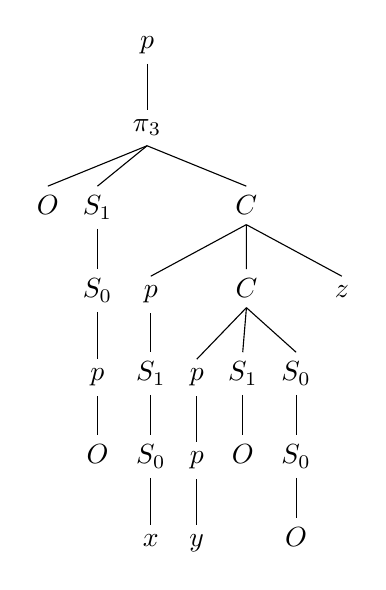
\begin{tikzpicture}
\Tree [.{$p$}
    [.{$\pi_3$}
        [.{$O$} ]
        [.{$S_1$}
            [.{$S_0$}
                [.{$p$}
                    [.{$O$} ]
                ]
            ]
        ]
        [.{$C$}
            [.{$p$}
                [.{$S_1$}
                    [.{$S_0$}
                        [.{$x$} ]
                    ]
                ]
            ]
            [.{$C$}
                [.{$p$}
                    [.{$p$}
                        [.{$y$} ]
                    ]
                ]
                [.{$S_1$}
                    [.{$O$} ]
                ]
                [.{$S_0$}
                    [.{$S_0$}
                        [.{$O$} ]
                    ]
                ]
            ]
            [.{$z$} ]
        ]
    ]
]
\end{tikzpicture}

  \caption{Syntax tree for function $
  p \Biggl(: 
    \pi_3\Biggl(: 
      O(:), 
      S_1\biggl(:
        S_0\Bigl(: 
          p\bigl(: 
            O(:)
          \bigr)
        \Bigr)
      \biggr),
      C \Biggl(:
        p \Bigl(:
          S_1 \bigl(:
            S_0(: x)
          \bigr)
        \Bigr),
        C\biggl(:
          p\bigl(:
            p(:y)
          \bigr),
          S_1 \bigl(:
            O(:)
          \bigr),
          S_0\Bigl(:
            S_0 \bigl(:
              O(:)
            \bigr)
          \Bigr),
          z
        \biggr)
      \Biggr)
    \Biggr)
  \Biggr)
$}
\end{figure}
\end{document}
